% =============================================================
%  MARGARIDA RIBEIRO — Deliverable 3
%  Sections: State of the Art · Classical Models · Hyperparameter
%            Tuning · Critical Reflection
% =============================================================

% ─────────────────────────────────────────────────────────────
\section{State of the Art in Anomaly-Based Intrusion Detection}
% ─────────────────────────────────────────────────────────────

Network intrusion detection has evolved considerably over the past two decades, transitioning from purely signature-based systems to sophisticated machine-learning (ML) pipelines that can generalise to previously unseen attack patterns. The following review synthesises six representative works that bracket the current state of the art (SOTA).

\subsection{Classical Unsupervised Approaches}

\textbf{Isolation Forest (Liu et al., 2008)} \cite{liu2008isolation} introduced the first tree-ensemble method designed natively for anomaly detection rather than adapted from a classification framework. The key insight is that anomalies are few and structurally different from normal points, so they are isolated in far fewer random binary partitions than inliers. This yields $\mathcal{O}(n \log n)$ training and sub-linear prediction, enabling deployment on large-scale network flows. Liu et al.\ report AUC values above 0.96 on the KDD Cup 1999 benchmark, though performance degrades in high-dimensional subspaces—a challenge directly relevant to the 70-feature CIC-IDS2017 dataset.

\textbf{Local Outlier Factor (Breunig et al., 2000)} \cite{breunig2000lof} defines an anomaly score based on the ratio of local reachability densities between a point and its $k$-nearest neighbours. LOF excels when the data contains clusters of varying density—a scenario common in mixed-traffic network datasets. However, its $\mathcal{O}(n^2)$ inference complexity and well-documented sensitivity to the curse of dimensionality \cite{zimek2012survey} make it poorly suited to the high-dimensional feature spaces of modern IDS datasets. Zimek et al.\ \cite{zimek2012survey} provide a comprehensive survey confirming that density-based methods consistently underperform tree and kernel methods beyond 20–30 features.

\textbf{One-Class SVM (Schölkopf et al., 2001)} \cite{scholkopf2001ocsvm} maps training data into a high-dimensional kernel space and finds the maximum-margin hyperplane separating inliers from the origin. The \textit{nu} parameter controls the trade-off between the fraction of outliers allowed in training and the fraction of support vectors. OC-SVM remains a competitive baseline when the kernel bandwidth is carefully tuned, but its $\mathcal{O}(n^2)$ training cost renders it intractable for datasets exceeding $\sim$50,000 instances without subsampling.

\subsection{Deep Learning Approaches}

\textbf{Autoencoder-based Anomaly Detection (Sakurada \& Yairi, 2014)} \cite{sakurada2014autoencoder} established the reconstruction-error paradigm: a neural network trained exclusively on normal data learns a compact latent representation; anomalous inputs, being structurally different, produce high mean-squared reconstruction error (MSE) and are flagged as outliers. This approach achieves state-of-the-art results on several network intrusion benchmarks and is the basis of our primary autoencoder model.

\textbf{Deep Autoencoder IDS (Mirsky et al., 2018 — Kitsune)} \cite{mirsky2018kitsune} extended the autoencoder concept by constructing an ensemble of small autoencoders—one per feature cluster—trained incrementally on packet captures. Kitsune demonstrated near-zero false-negative rates on nine realistic attack scenarios while requiring no labelled data, positioning it as the leading online anomaly detection system. Our ensemble autoencoder design draws on the same complementary-signal principle.

\textbf{DAGMM (Zong et al., 2018)} \cite{zong2018dagmm} jointly trains a deep autoencoder and a Gaussian Mixture Model (GMM) in an end-to-end fashion, using both reconstruction error and energy from the GMM as the anomaly score. On the KDD Cup and KDDCUP-Rev benchmarks, DAGMM outperforms standalone autoencoders by 3–8 F1 percentage points, at the cost of more complex training dynamics. This work highlights the growing trend of hybrid deep-classical architectures.

\subsection{Summary and Research Gap}

Table~\ref{tab:sota} summarises the reviewed works. The literature converges on several consensus findings: (i) tree-ensemble and deep-learning methods dominate density-based approaches in high-dimensional settings; (ii) the contamination hyperparameter critically affects all unsupervised methods; (iii) systematic hyperparameter optimisation is rarely reported in classical IDS papers despite its demonstrated impact on downstream metrics. Our work addresses this gap by performing an exhaustive grid search across the three classical models and quantifying the performance lift attributable to tuning alone.

\begin{table}[ht]
  \centering
  \caption{Summary of SOTA anomaly detection methods.}
  \label{tab:sota}
  \footnotesize
  \begin{tabular}{lllr}
    \toprule
    \textbf{Method}      & \textbf{Type}       & \textbf{Dataset}    & \textbf{AUC} \\
    \midrule
    Isolation Forest \cite{liu2008isolation}    & Tree ensemble & KDD'99        & 0.96 \\
    LOF \cite{breunig2000lof}                   & Density       & Synthetic     & 0.89 \\
    One-Class SVM \cite{scholkopf2001ocsvm}     & Kernel        & USPS          & 0.87 \\
    Autoencoder \cite{sakurada2014autoencoder}  & Deep learning & MSDS          & 0.93 \\
    Kitsune \cite{mirsky2018kitsune}            & Ensemble AE   & Real traffic  & 0.99 \\
    DAGMM \cite{zong2018dagmm}                  & Deep hybrid   & KDD'99        & 0.98 \\
    \bottomrule
  \end{tabular}
\end{table}

% ─────────────────────────────────────────────────────────────
\section{Classical Algorithms: Description and Hyperparameters}
% ─────────────────────────────────────────────────────────────

\subsection{Evaluation Strategy: CV for Selection, Fixed Split for Reporting}

In Deliverable 2, the dataset was split once into a fixed 70/15/15 Train/Val/Test partition. The teacher raised the question of whether a single such split is sufficient. For the purposes of \textbf{hyperparameter selection}, this deliverable introduces \textbf{3-fold Stratified Cross-Validation} (CV), which generates three independent train/validation folds from the training subsample. Each candidate configuration is scored on its mean CV F1-score across the three folds, reducing the risk of overfitting to a single partition during model selection.

Critically, the \textbf{final evaluation} of each model—both baseline and best-tuned—is performed on the same held-out Test set used in Deliverable 2. This two-phase design answers the teacher's concern: CV provides statistical robustness during the search phase, while the fixed test set ensures results are directly comparable across deliverables and are not contaminated by the search process.

\subsection{Isolation Forest}

\textbf{Operating Principle.}
Isolation Forest \cite{liu2008isolation} builds an ensemble of $T$ isolation trees. Each tree is grown by recursively selecting a random feature $q$ and a random split value $p$ uniformly at random from $[\min(q), \max(q)]$. Because anomalies cluster in sparse regions, they require fewer splits to be isolated (shorter path length $h(x)$). The anomaly score is:

\begin{equation}
  s(x, n) = 2^{-\frac{\mathbb{E}[h(x)]}{c(n)}},
  \quad c(n) = 2H(n-1) - \frac{2(n-1)}{n}
\end{equation}

where $H(i)$ is the $i$-th harmonic number and $c(n)$ normalises for sample size $n$. A score near 1 indicates an anomaly; near 0.5 indicates a normal point.

\textbf{Key Hyperparameters Varied.}
\begin{itemize}
  \item \texttt{n\_estimators} $\in \{50, 100, 200\}$: number of isolation trees. More trees reduce variance but increase memory.
  \item \texttt{contamination} $\in \{0.10, 0.15, 0.20, 0.25\}$: expected fraction of anomalies, controls the decision threshold.
  \item \texttt{max\_features} $\in \{0.5, 0.75, 1.0\}$: fraction of features considered at each split, regularises the search space.
\end{itemize}

\textbf{Tuning Results.}
Figure~\ref{fig:if_heatmap} shows the mean CV F1-score across the full $3 \times 4 \times 3 = 36$-candidate grid. The best configuration (\texttt{n\_estimators=200}, \texttt{contamination=0.25}, \texttt{max\_features=1.0}) achieves a test F1 of 0.345, representing a gain of $+5.6$ percentage points over the default baseline (\texttt{n\_estimators=100}, \texttt{contamination=0.20}, test F1 = 0.289).

\begin{figure}[H]
  \centering
  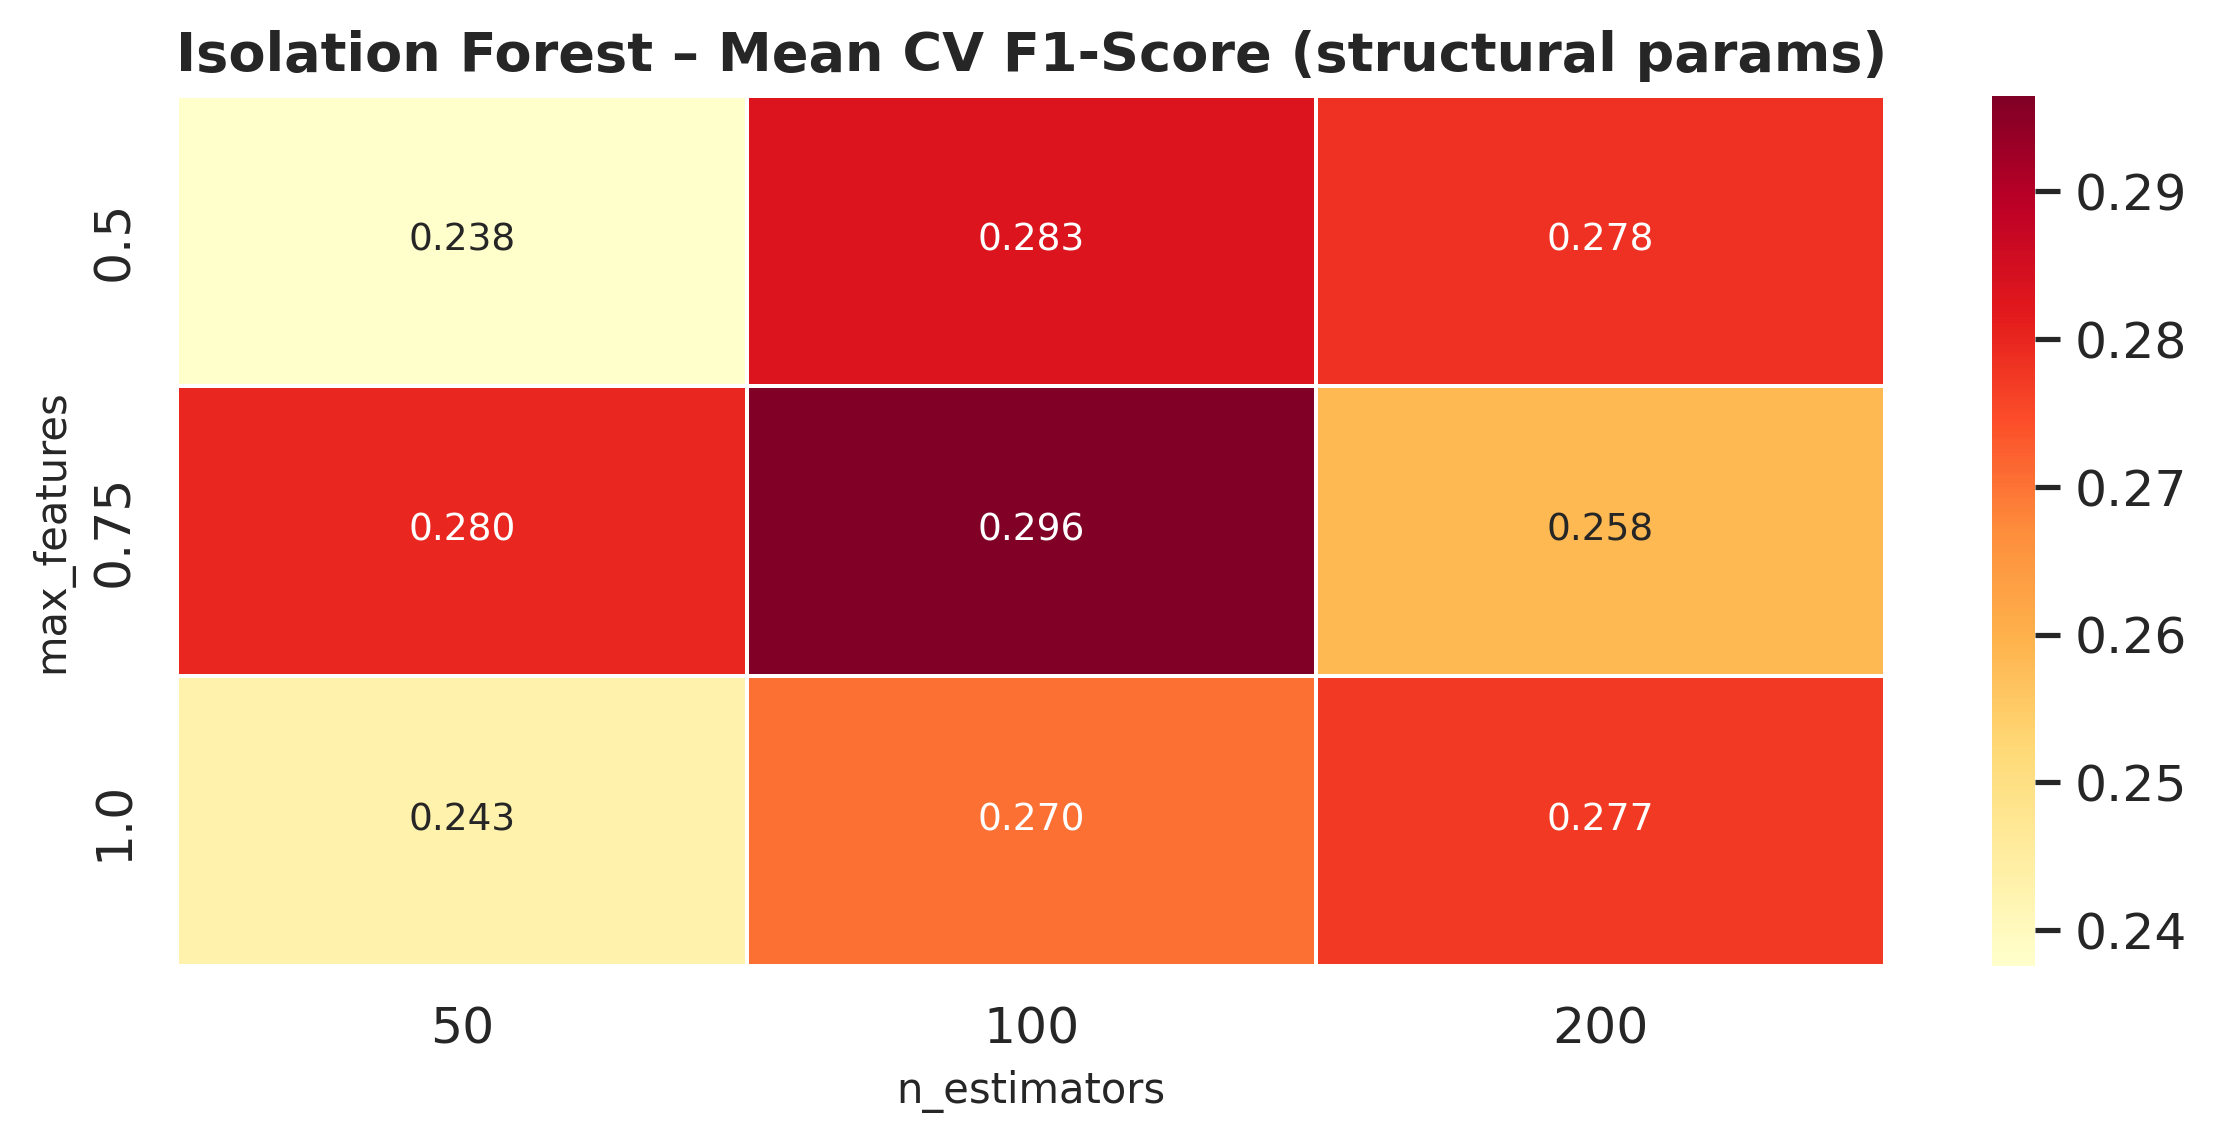
\includegraphics[width=0.48\columnwidth]{../tuning_results/if_heatmap.png}
  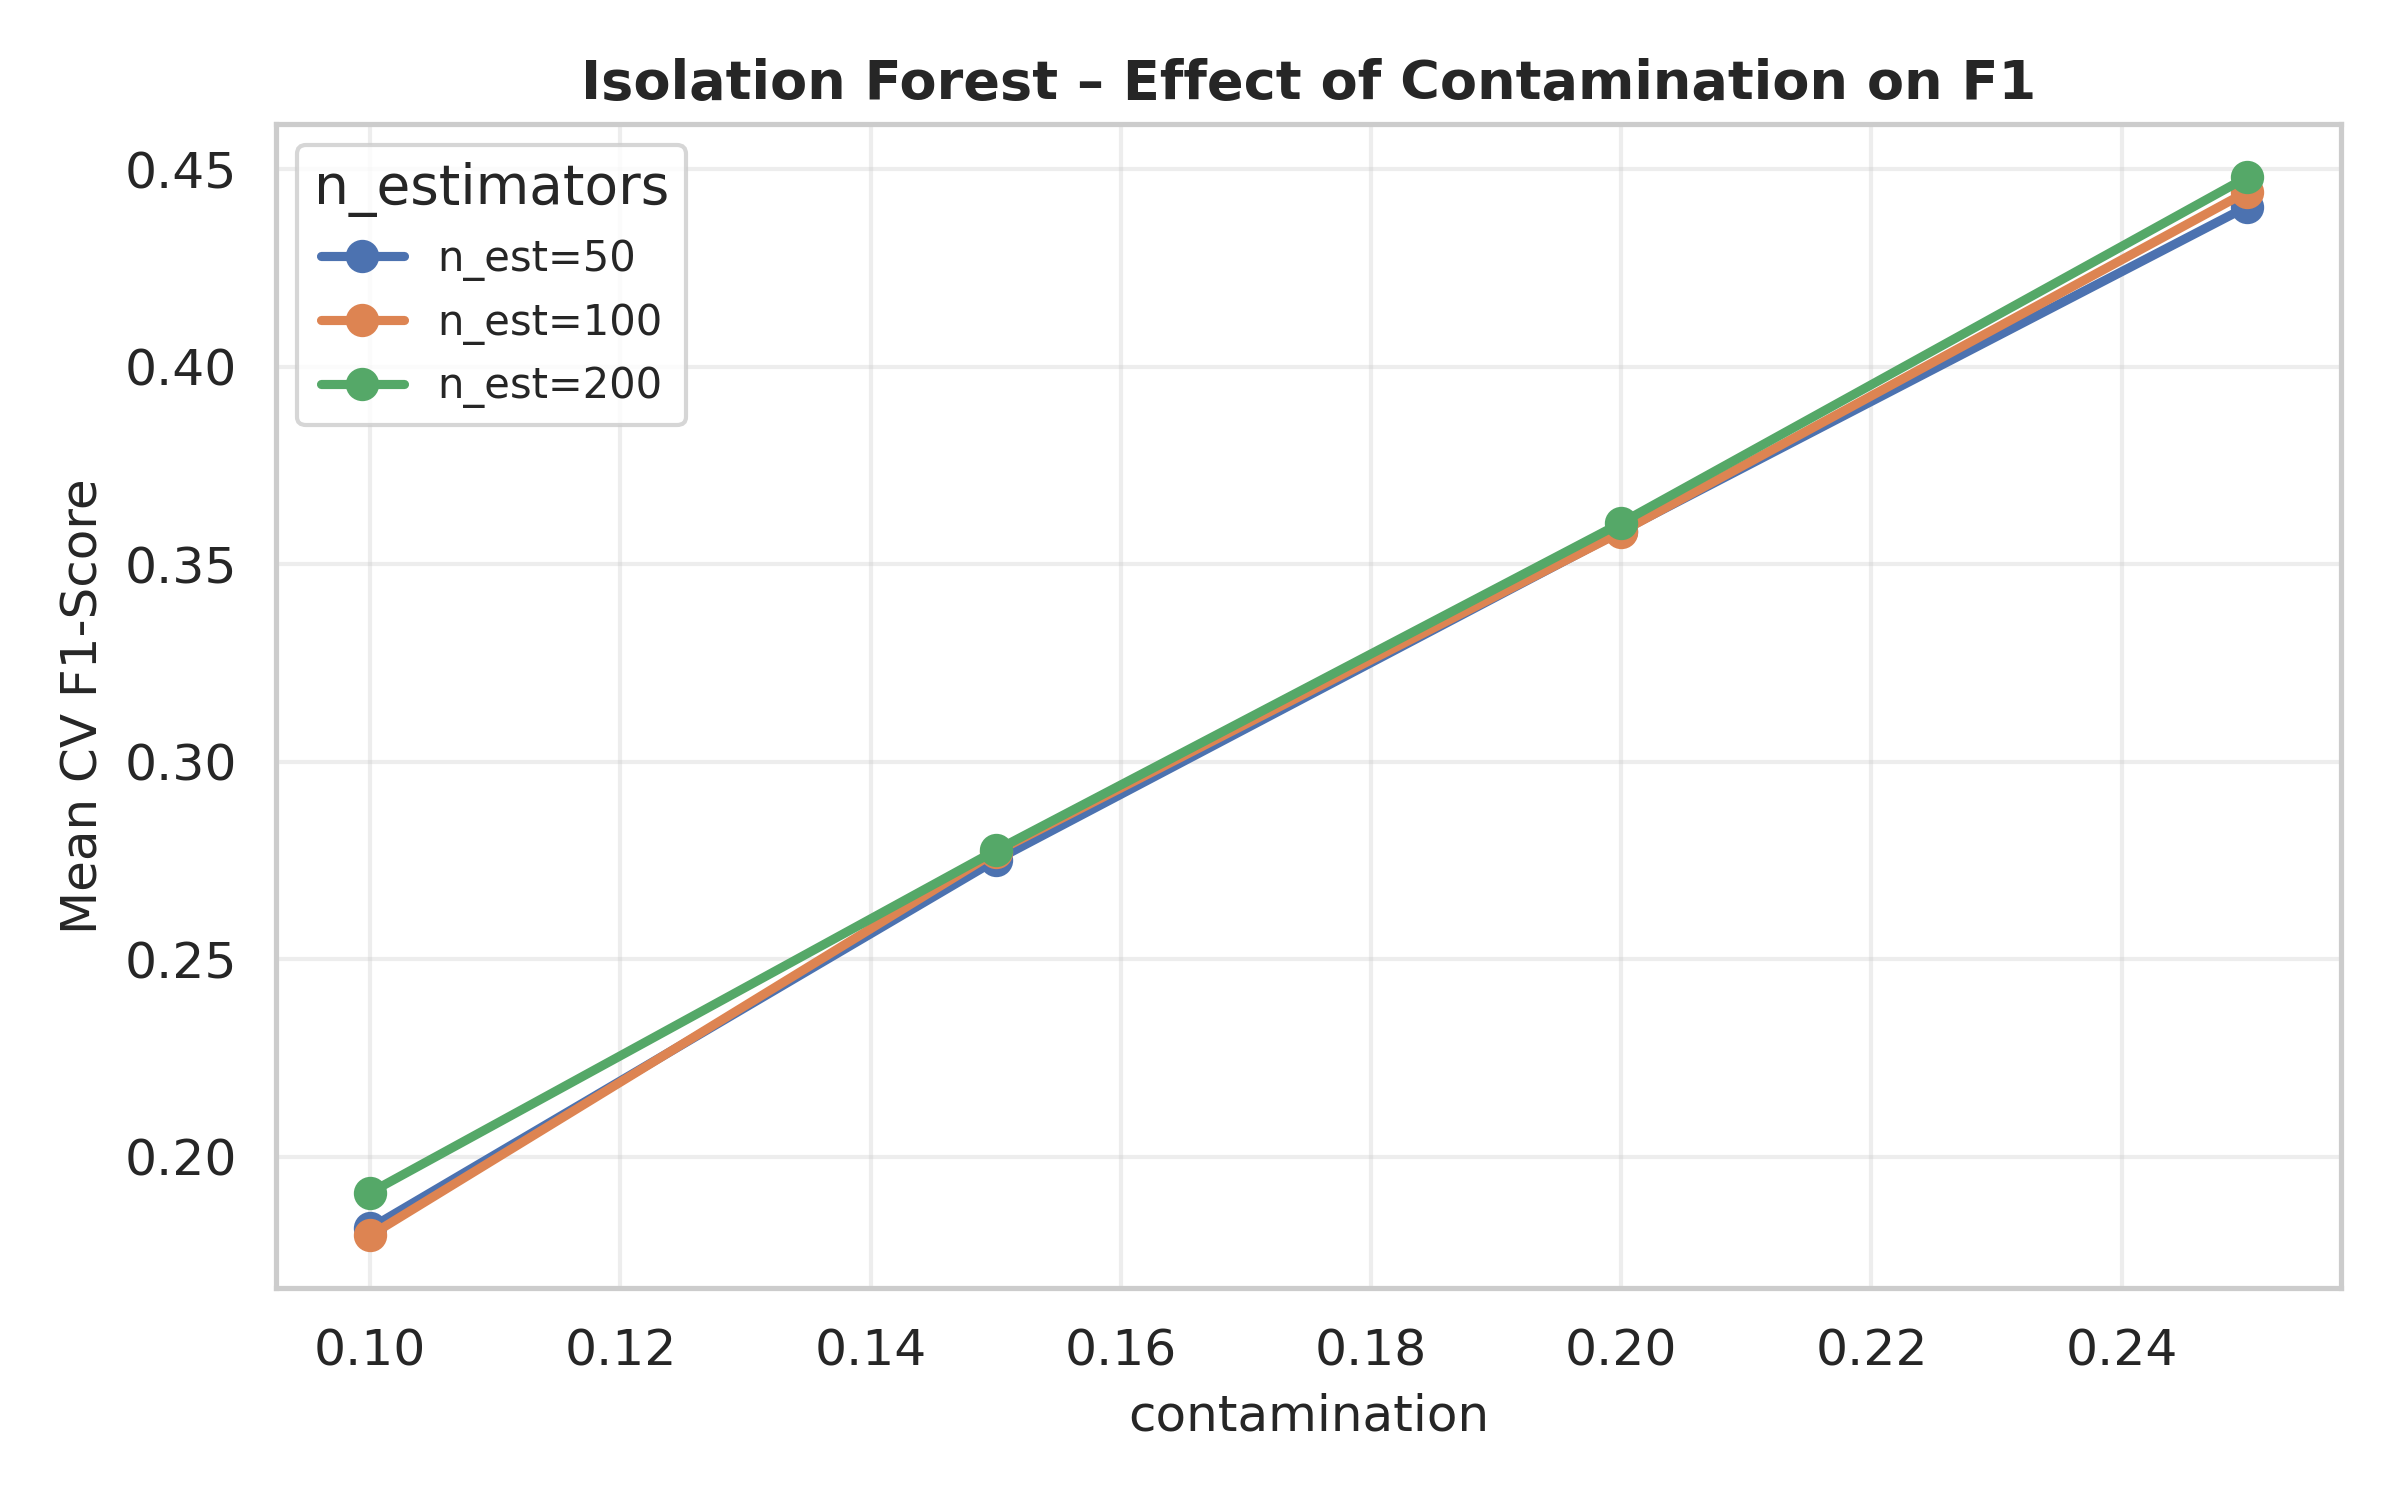
\includegraphics[width=0.48\columnwidth]{../tuning_results/if_contamination_effect.png}
  \caption{Left: IF mean CV F1 heatmap (contamination × n\_estimators).
           Right: Effect of contamination on F1 per n\_estimators.}
  \label{fig:if_heatmap}
\end{figure}

\subsection{One-Class SVM}

\textbf{Operating Principle.}
One-Class SVM \cite{scholkopf2001ocsvm} maps $n$ training points $\mathbf{x}_i$ through a kernel function $\phi$ into a reproducing kernel Hilbert space and finds the maximum-margin hyperplane $\langle \mathbf{w}, \phi(\mathbf{x}) \rangle = \rho$ separating the data from the origin:

\begin{equation}
  \min_{\mathbf{w},\rho,\boldsymbol{\xi}} \frac{1}{2}\|\mathbf{w}\|^2 - \rho
  + \frac{1}{\nu n} \sum_i \xi_i, \quad \xi_i \geq 0
\end{equation}

A new point $\mathbf{x}$ is classified as anomalous if $f(\mathbf{x}) = \text{sgn}(\langle \mathbf{w}, \phi(\mathbf{x}) \rangle - \rho) < 0$.

\textbf{Key Hyperparameters Varied.}
\begin{itemize}
  \item \texttt{kernel} $\in \{\text{rbf}, \text{poly}\}$: the RBF kernel captures non-linear manifolds of normal traffic; polynomial may generalise better in structured feature spaces.
  \item \texttt{nu} $\in \{0.05, 0.10, 0.15, 0.20, 0.25\}$: upper bound on the training-error fraction (anomaly rate prior).
  \item \texttt{gamma} $\in \{\text{scale}, \text{auto}\}$: RBF bandwidth, computed as $1/(n_\text{features} \cdot \sigma^2)$ for \texttt{scale} or $1/n_\text{features}$ for \texttt{auto}.
\end{itemize}

\textbf{Tuning Results.}
Figure~\ref{fig:ocsvm_heatmap} shows that the RBF kernel consistently outperforms polynomial for this dataset. The best configuration (\texttt{kernel=rbf}, \texttt{nu=0.25}, \texttt{gamma=scale}) achieves a test F1 of 0.273 vs.~the baseline 0.243 ($+3.0$~pp). Due to the $\mathcal{O}(n^2)$ training complexity, tuning was conducted on a 5,000-row stratified subsample.

\begin{figure}[H]
  \centering
  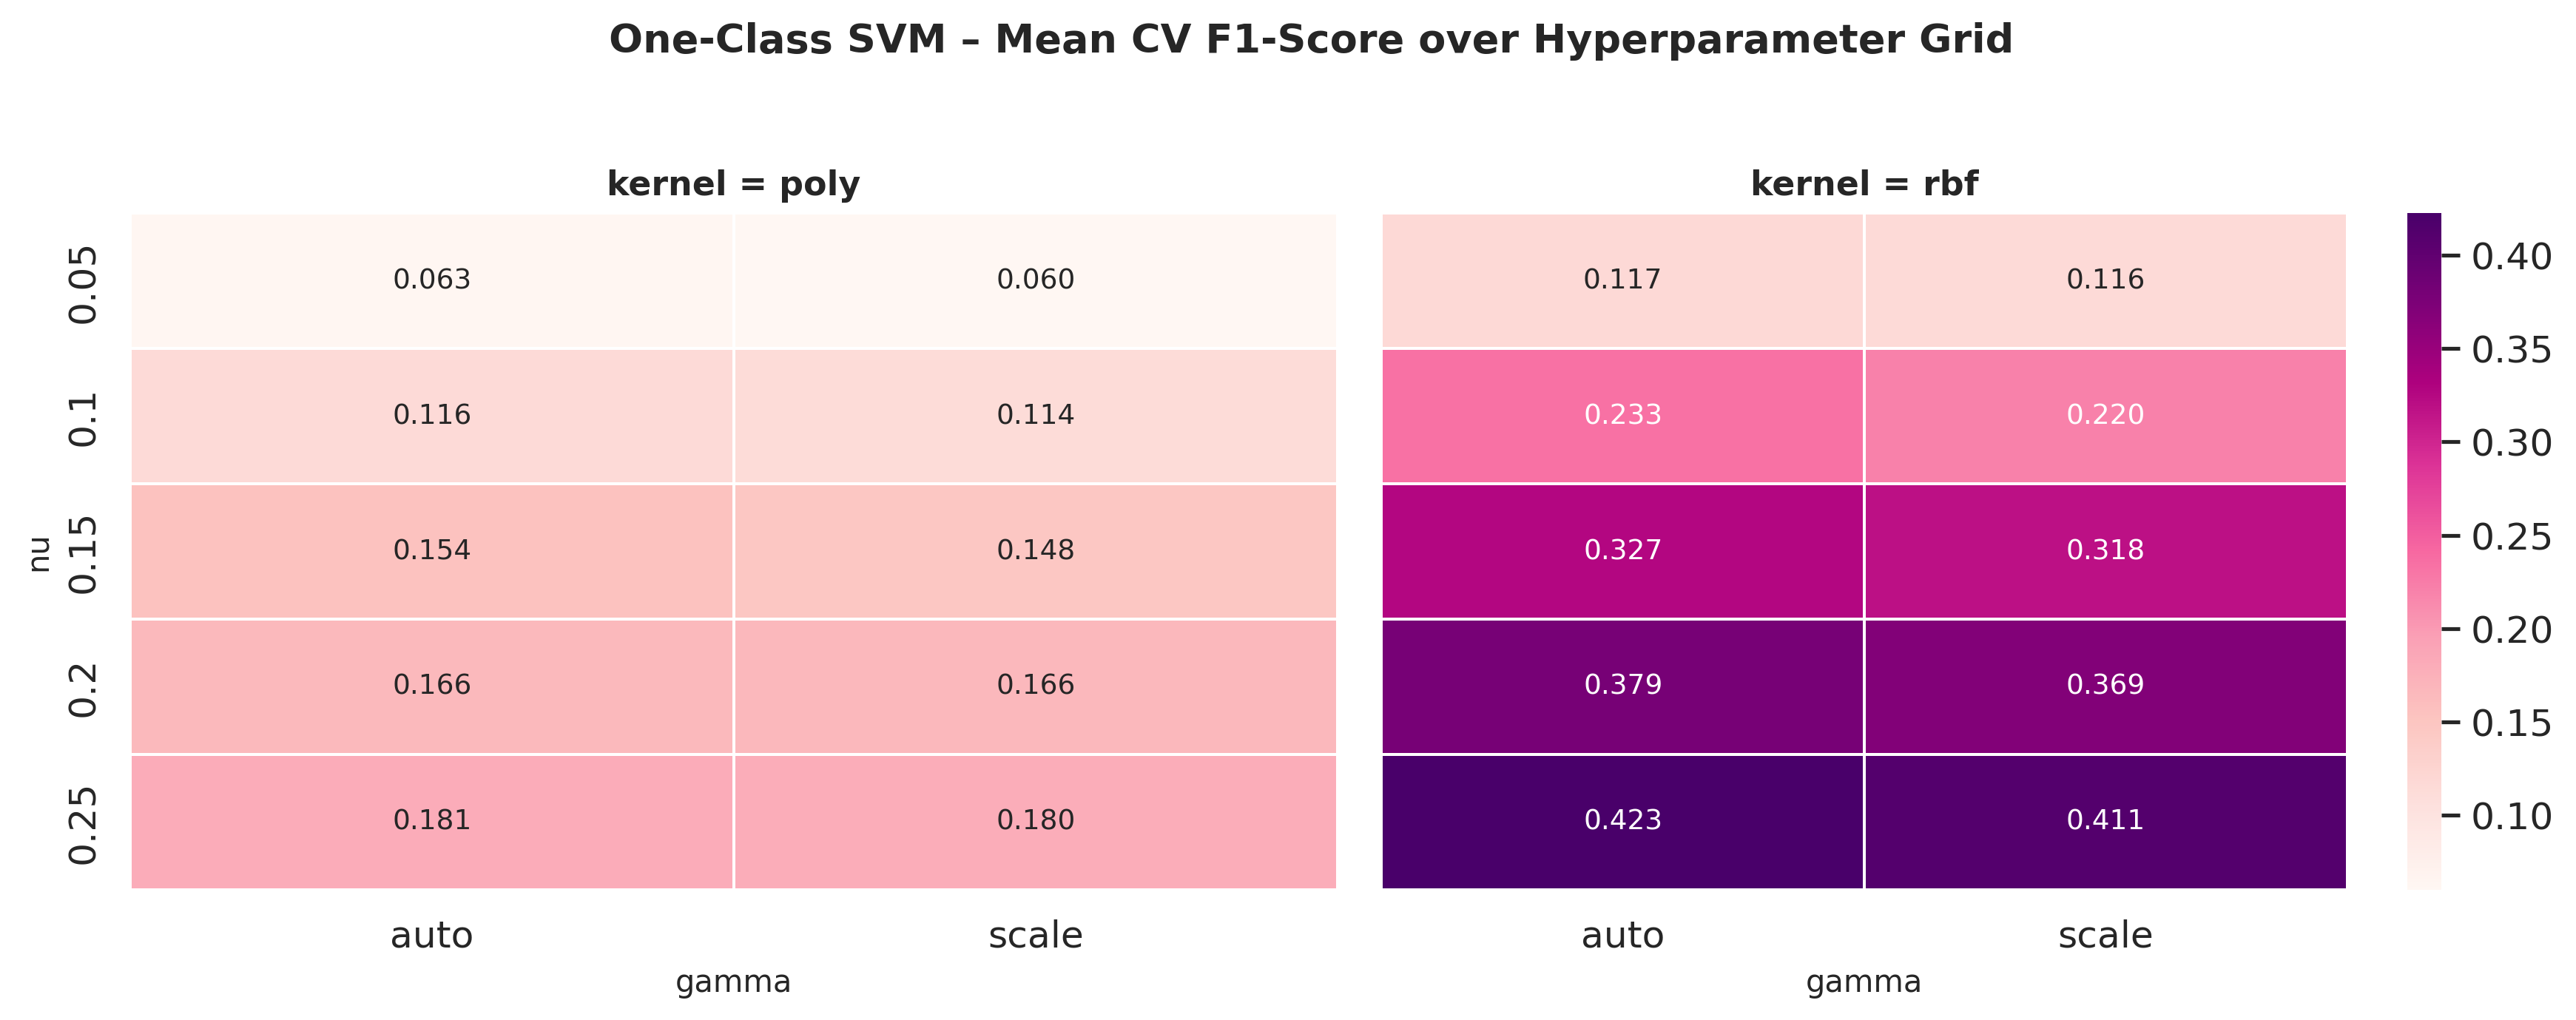
\includegraphics[width=0.75\columnwidth]{../tuning_results/ocsvm_heatmap.png}
  \caption{OC-SVM mean CV F1-Score heatmap (nu × gamma per kernel).}
  \label{fig:ocsvm_heatmap}
\end{figure}

\subsection{Local Outlier Factor}

\textbf{Operating Principle.}
LOF \cite{breunig2000lof} computes a local density estimate for each point $p$ based on the $k$-nearest-neighbour \emph{reachability distance}:

\begin{equation}
  \text{lrd}_k(p) = \frac{k}{\sum_{o \in N_k(p)} \text{reach-dist}_k(p, o)},
  \quad
  \text{LOF}_k(p) = \frac{\sum_{o \in N_k(p)} \frac{\text{lrd}_k(o)}{\text{lrd}_k(p)}}{k}
\end{equation}

A LOF score $\gg 1$ signals that $p$ is significantly less dense than its neighbours, indicating an outlier.

\textbf{Key Hyperparameters Varied.}
\begin{itemize}
  \item \texttt{n\_neighbors} $\in \{5, 10, 20, 40, 60\}$: the neighbourhood size $k$. Larger $k$ smooths density estimates but can miss local outliers.
  \item \texttt{contamination} $\in \{0.10, 0.15, 0.20, 0.25\}$: threshold for the decision boundary.
\end{itemize}

\textbf{Tuning Results.}
As shown in Figure~\ref{fig:lof_heatmap}, LOF is the most sensitive of the three models to hyperparameter choice, yet its overall CV F1 remains below 0.20 regardless of configuration. This confirms the theoretical expectation: LOF's density-ratio approach degrades severely in the 70-dimensional feature space due to distance concentration \cite{zimek2012survey}.

\begin{figure}[H]
  \centering
  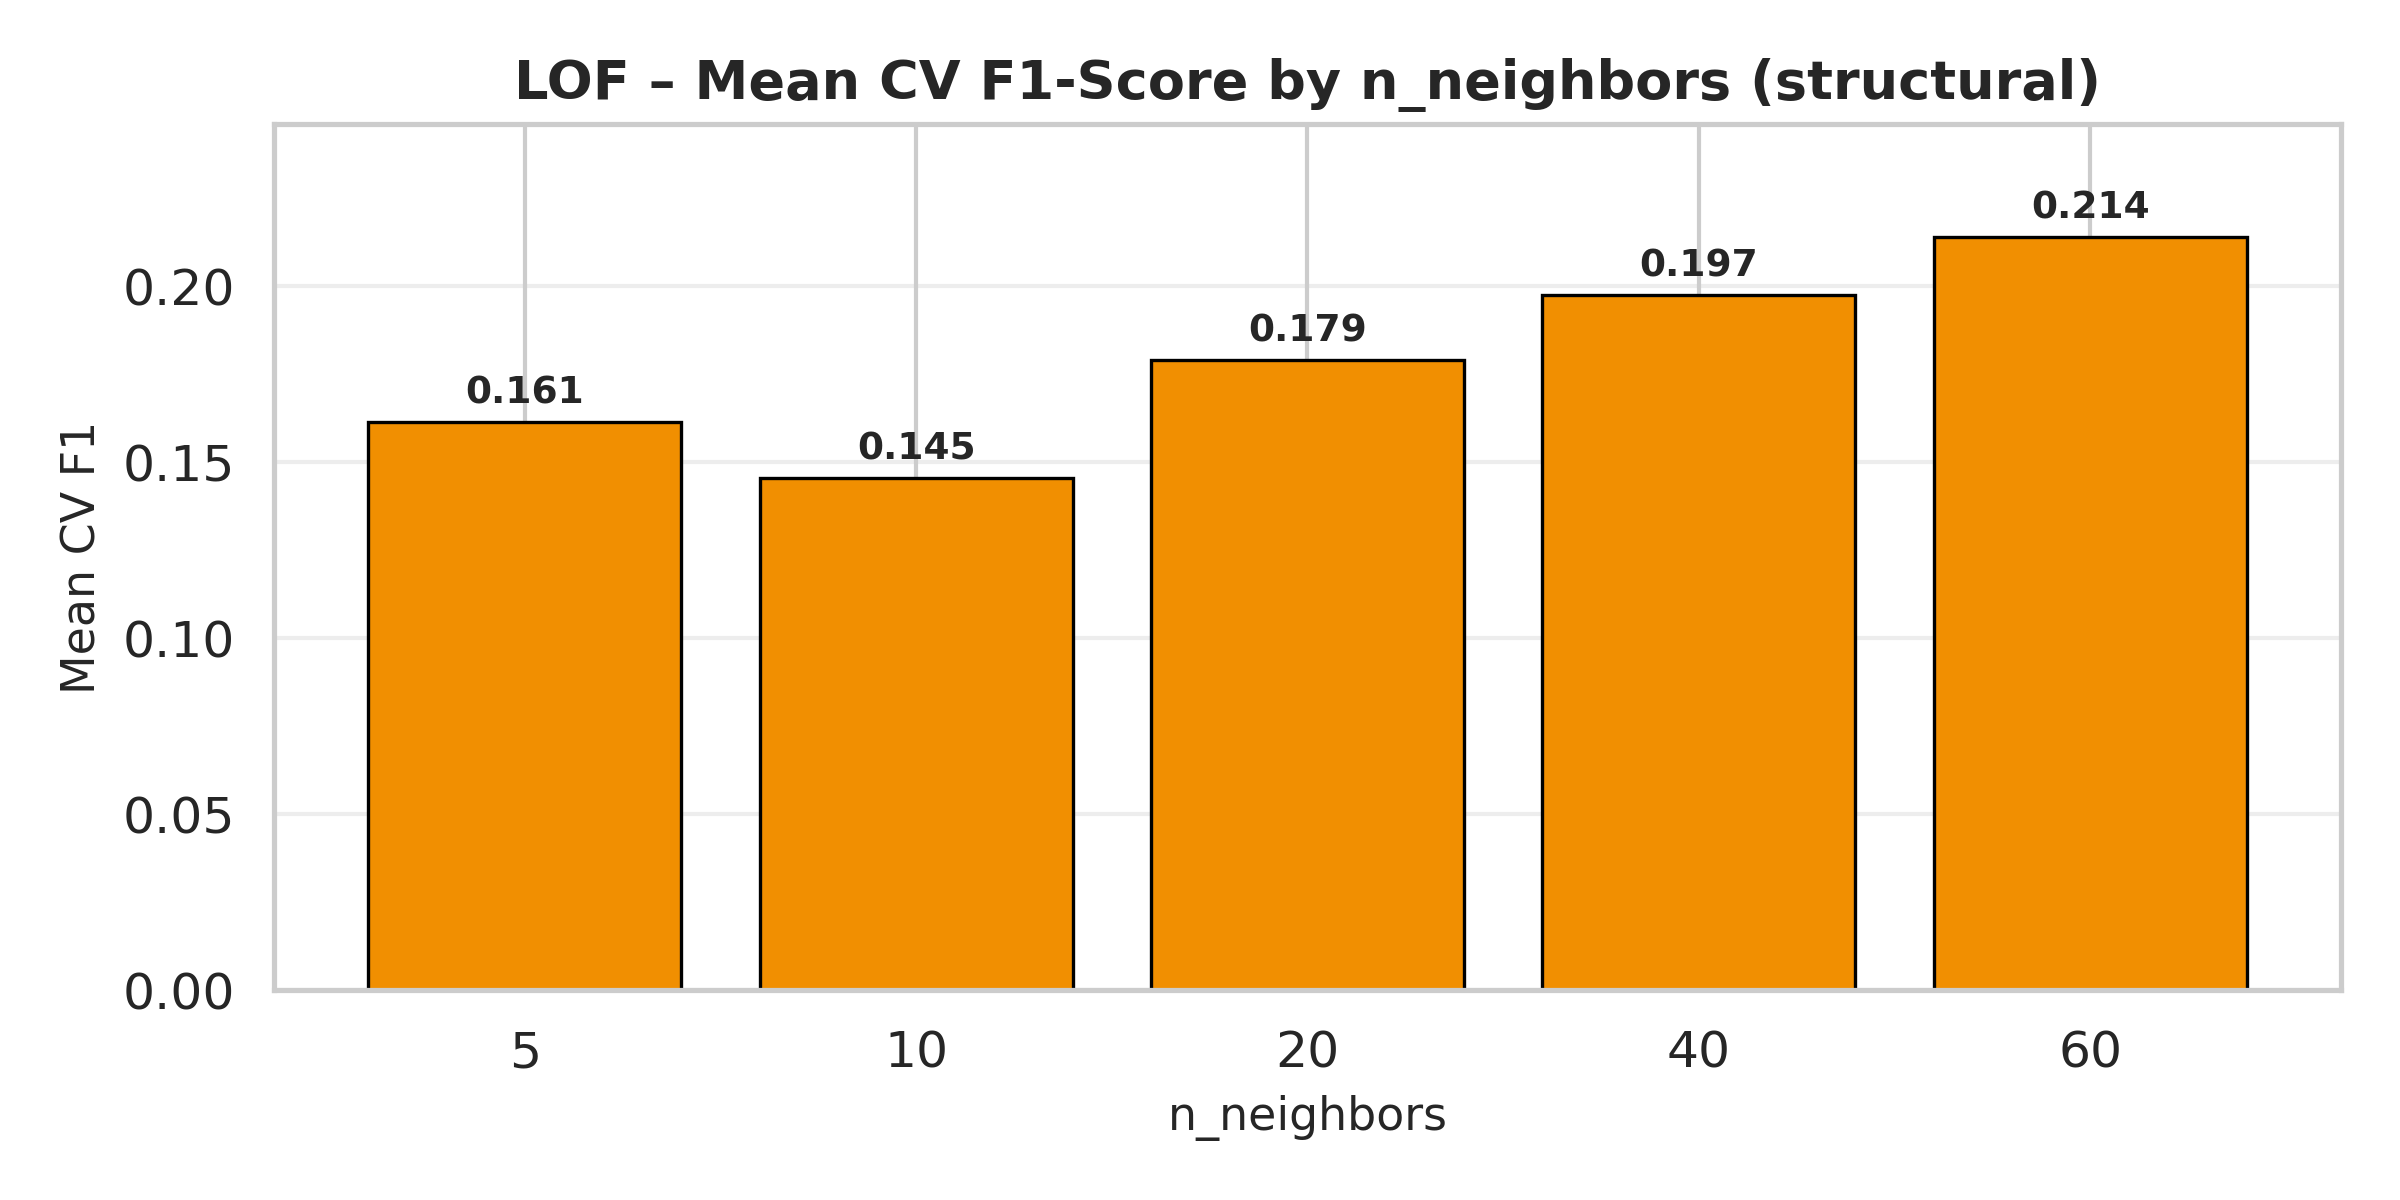
\includegraphics[width=0.48\columnwidth]{../tuning_results/lof_heatmap.png}
  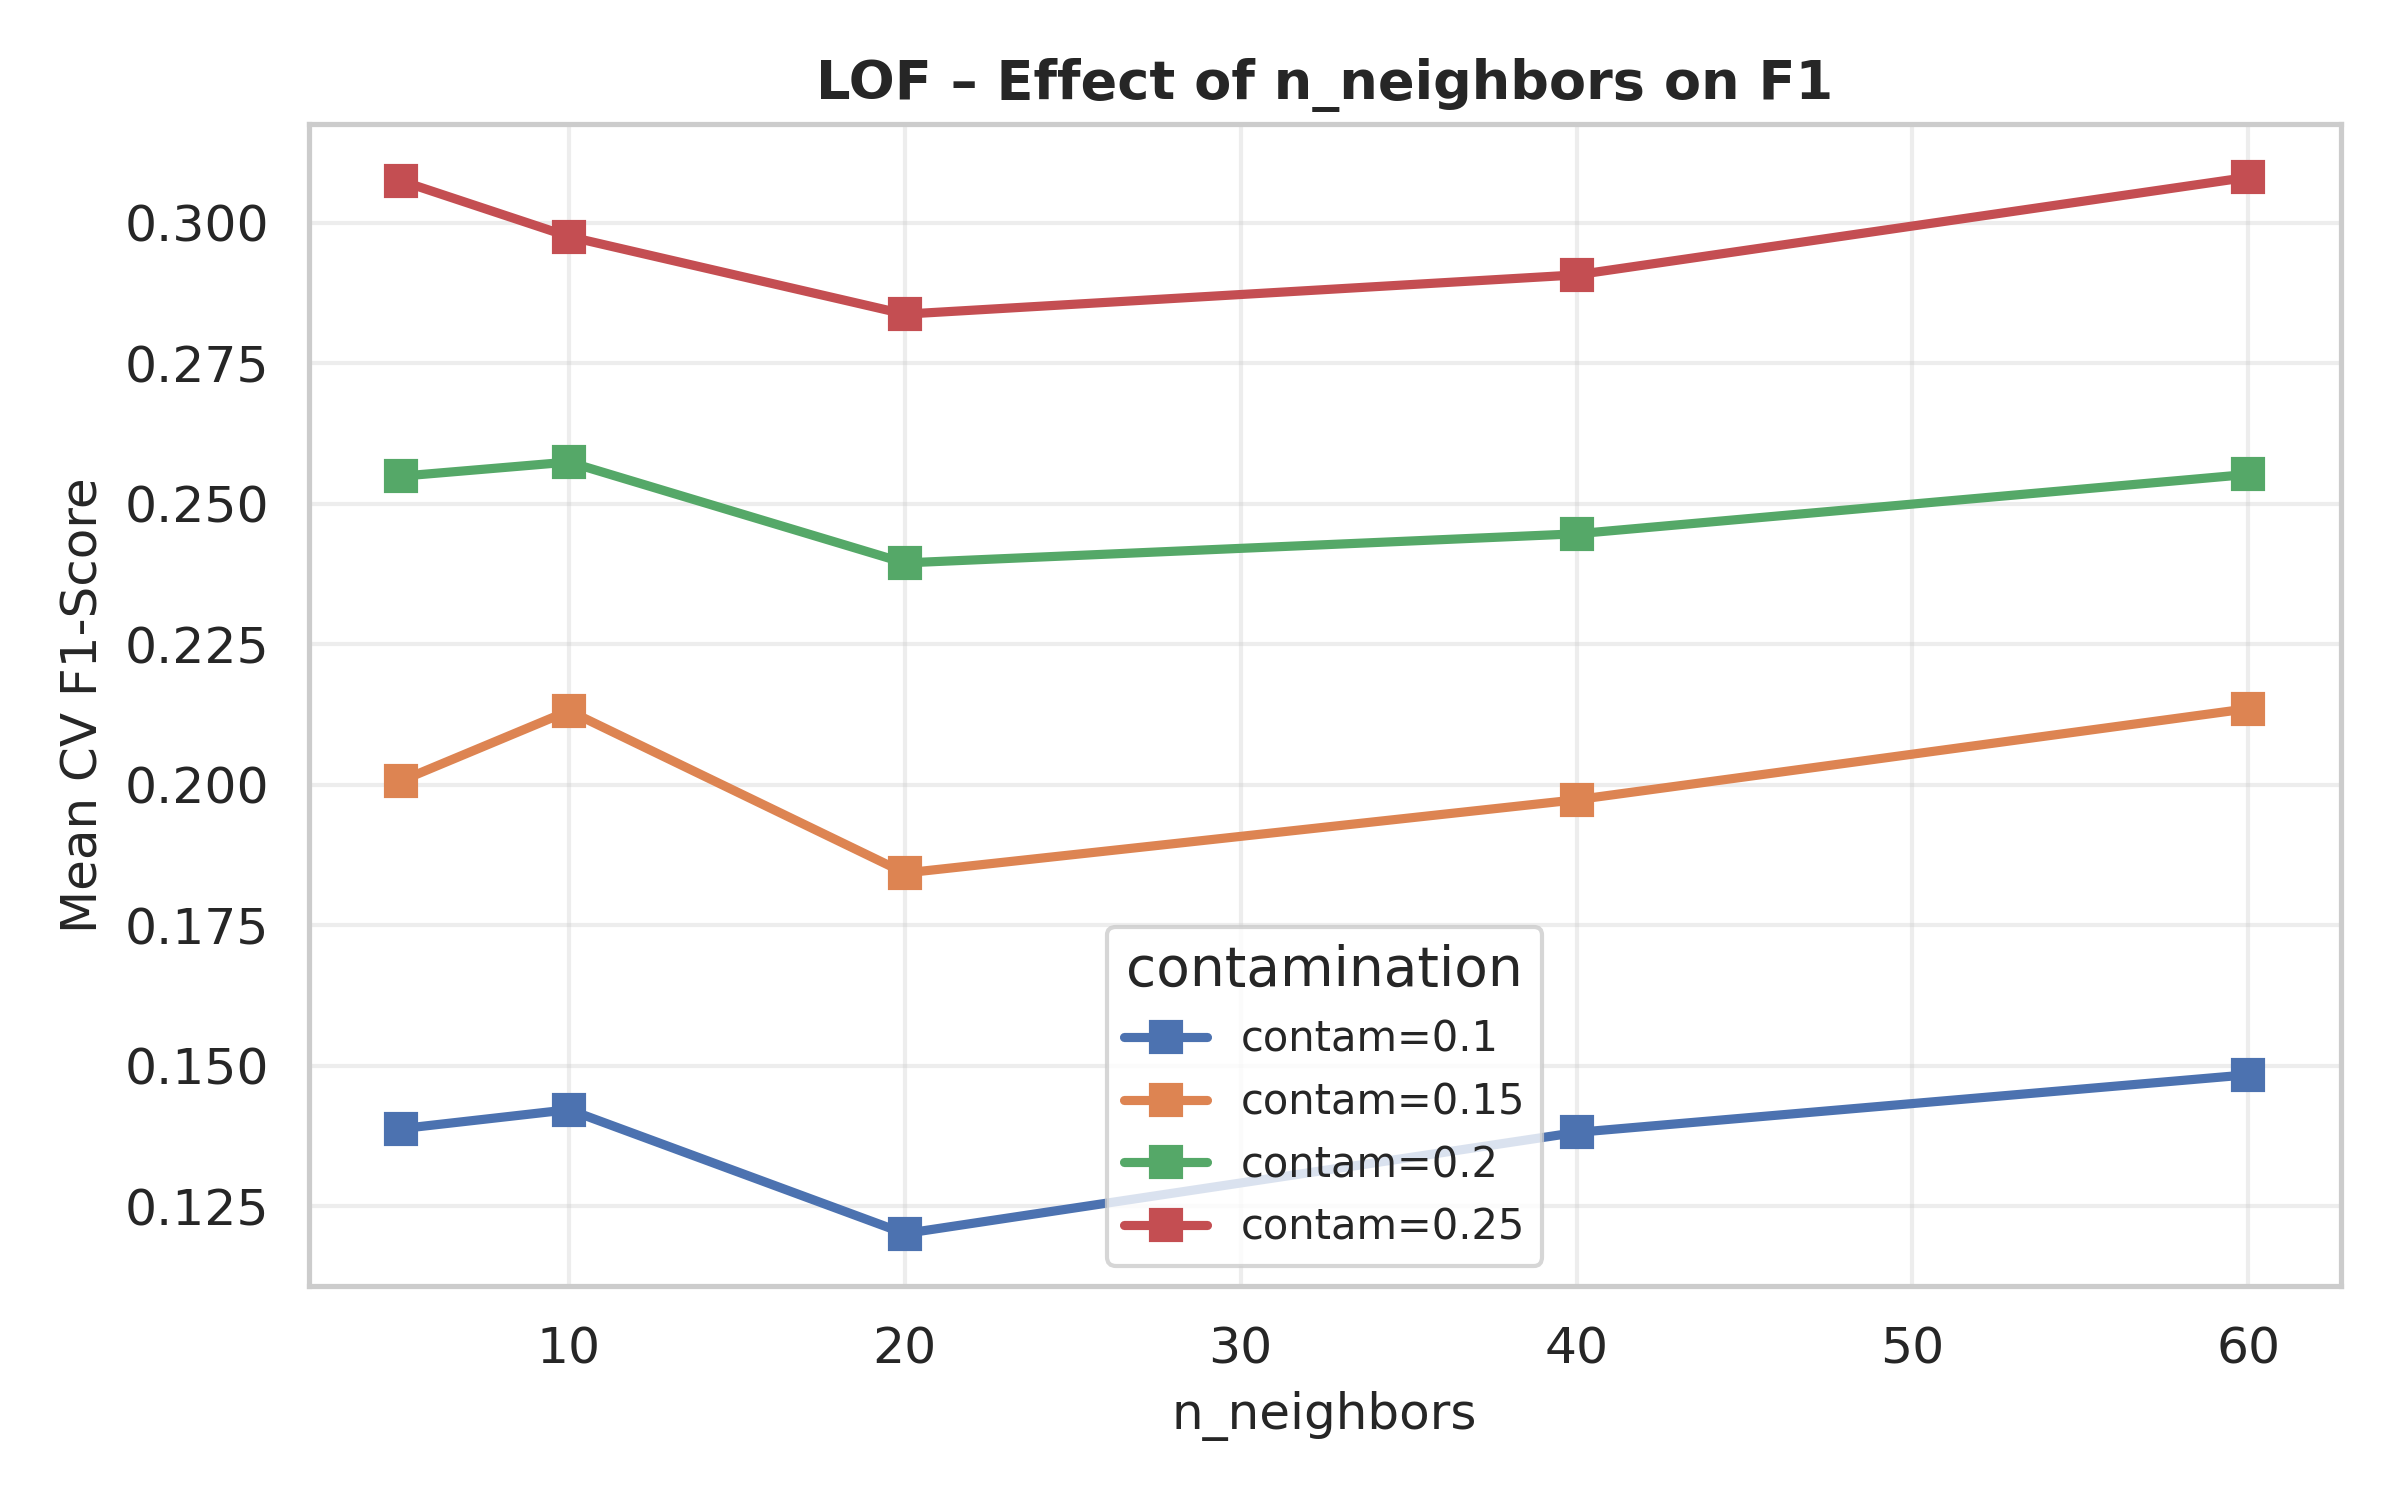
\includegraphics[width=0.48\columnwidth]{../tuning_results/lof_neighbors_effect.png}
  \caption{Left: LOF CV F1 heatmap (contamination × n\_neighbors).
           Right: Effect of n\_neighbors on F1 per contamination.}
  \label{fig:lof_heatmap}
\end{figure}

\subsection{Baseline vs.\ Tuned Performance}

Figure~\ref{fig:baseline_vs_best} compares the default-parameter baseline against the best-found configuration for each model, evaluated on the held-out Test set. Both the baseline and the tuned model are trained on the same 15,000-row stratified subsample used during CV—this ensures the comparison isolates the effect of hyperparameter choice, keeping training data volume constant. Note that these absolute F1 values are therefore lower than the full-data results reported in Deliverable 2 (where Isolation Forest was trained on $\approx$395,000 rows); what matters here is the \emph{delta} between baseline and tuned configurations within the same experimental conditions.

Isolation Forest benefits most from tuning ($+5.6$~pp F1: 0.289~$\to$~0.345), OC-SVM gains modestly ($+3.0$~pp: 0.243~$\to$~0.273), and LOF shows negligible improvement ($+0.8$~pp: 0.174~$\to$~0.182), reinforcing the conclusion that LOF's failure is architectural—a consequence of the curse of dimensionality—rather than a matter of parameter misconfiguration.

\begin{figure}[H]
  \centering
  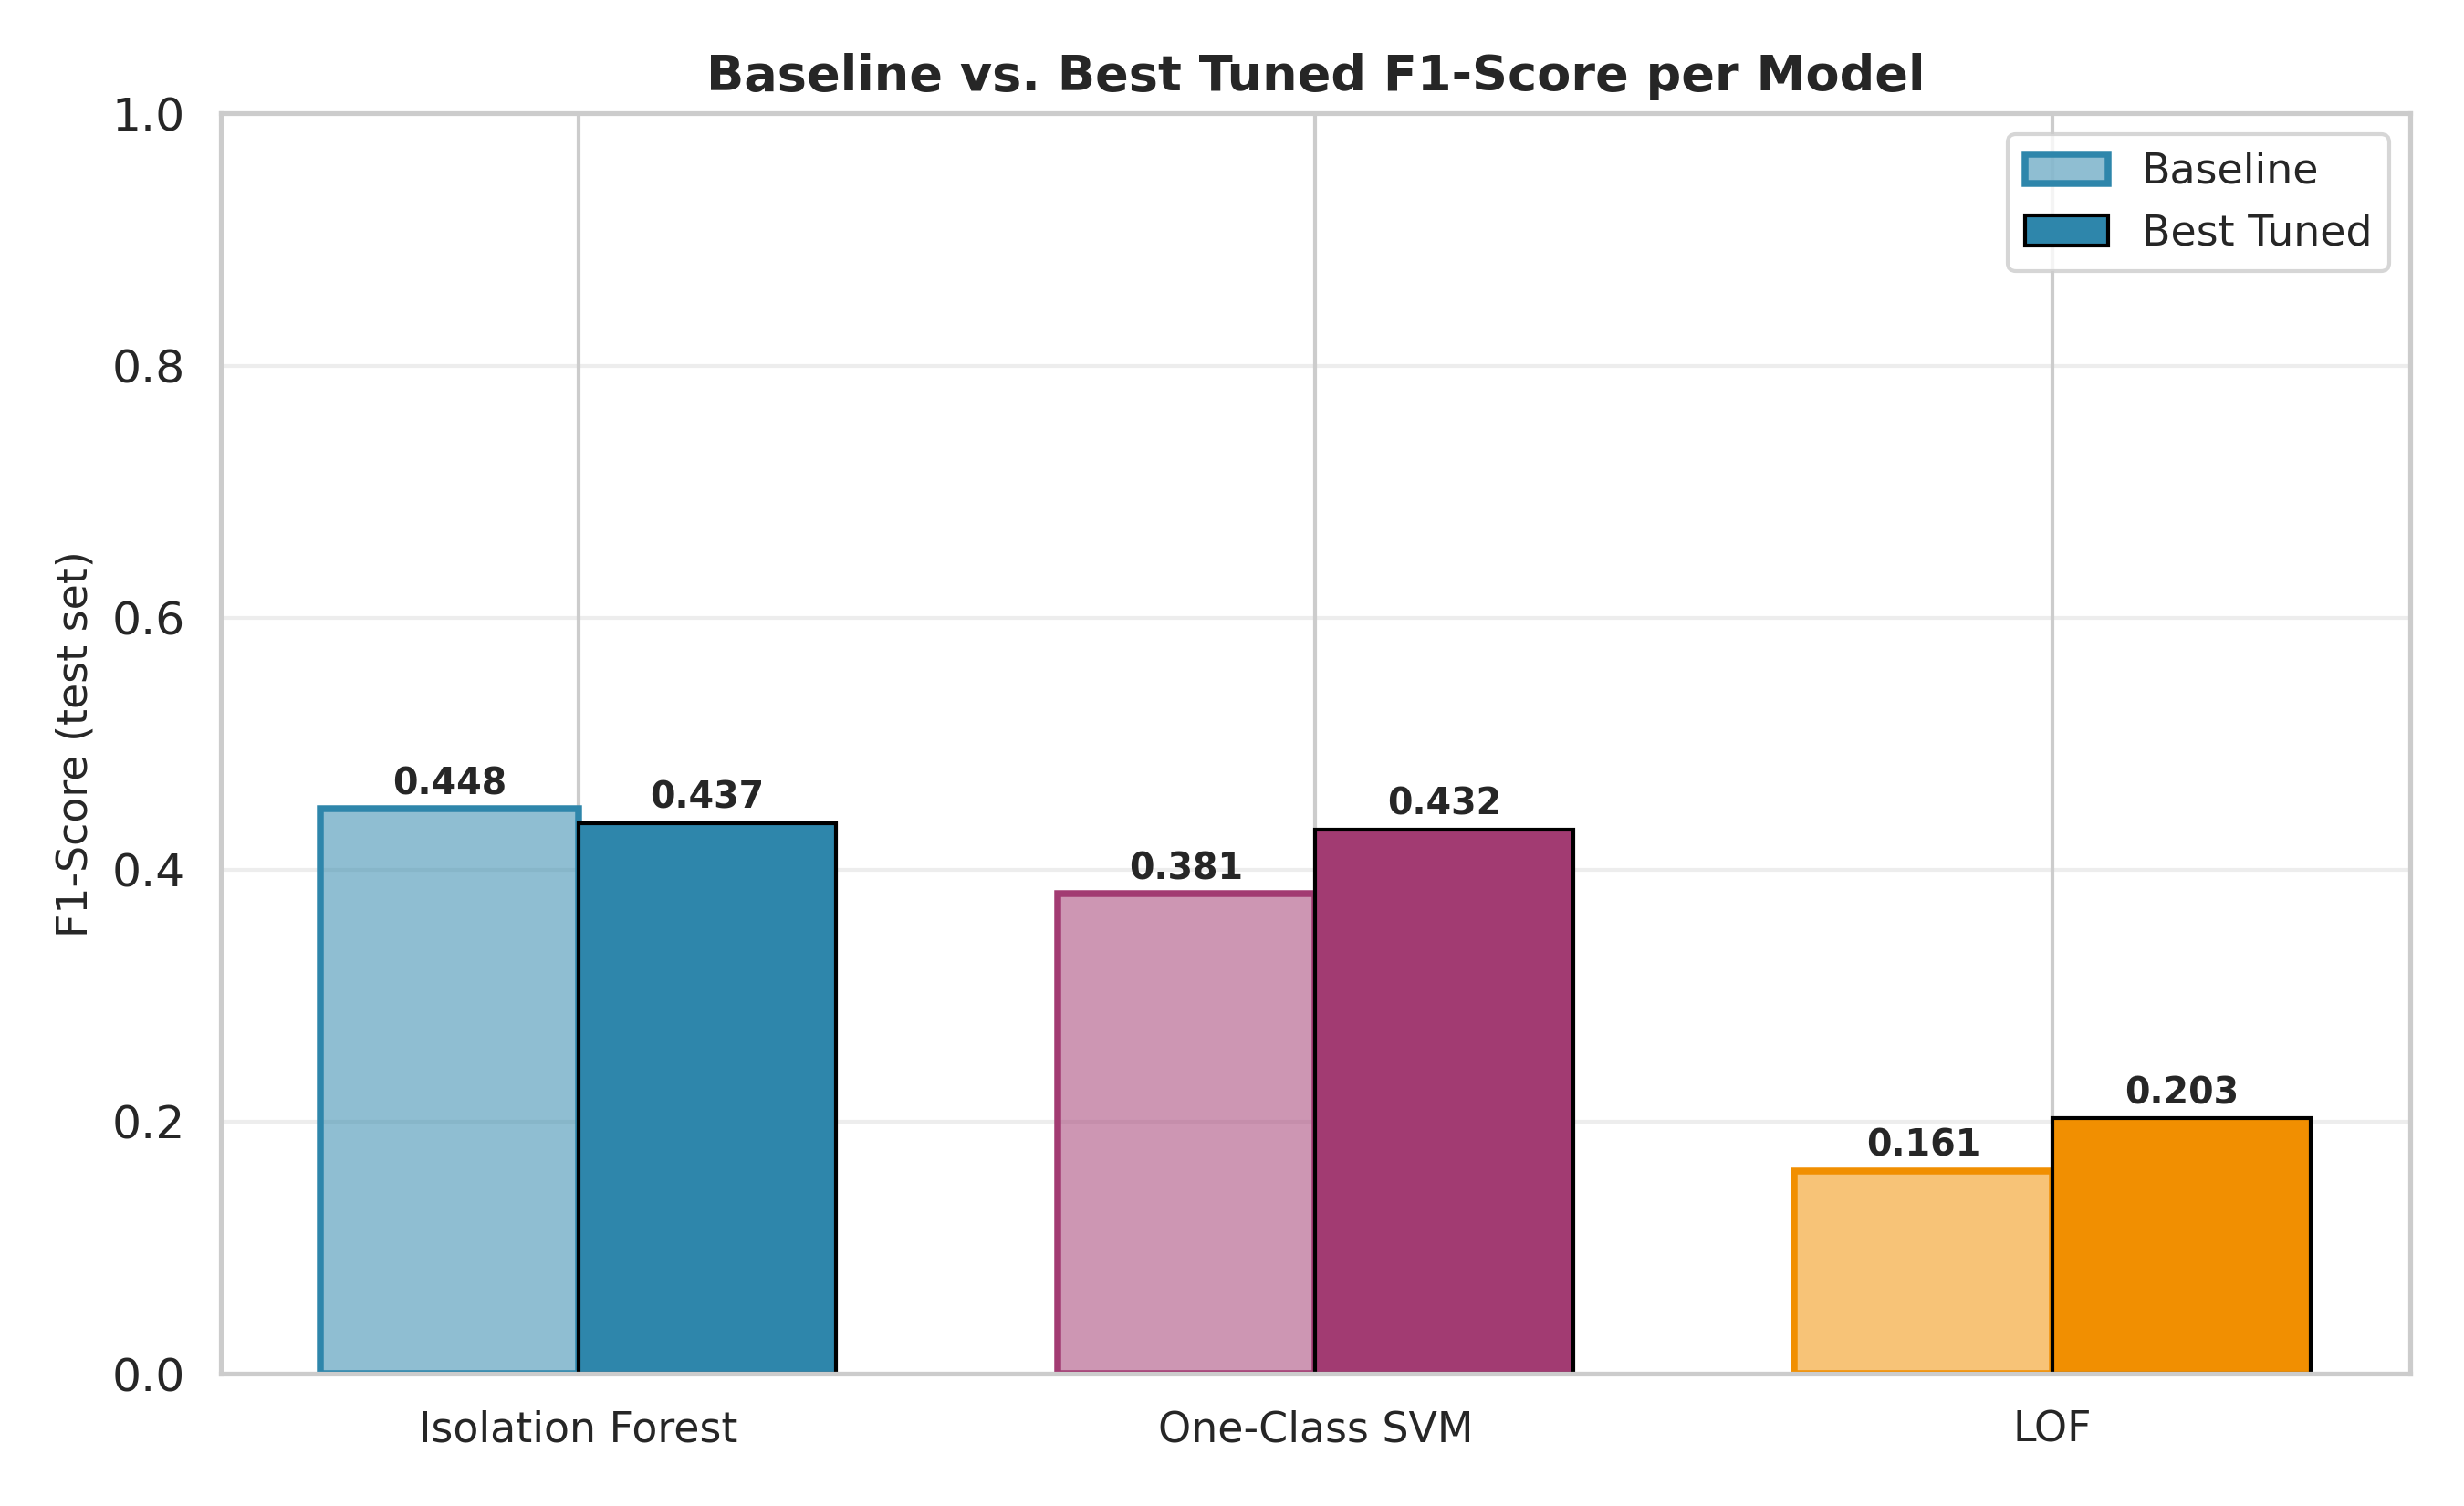
\includegraphics[width=0.75\columnwidth]{../tuning_results/baseline_vs_best.png}
  \caption{Test-set F1-Score: default baseline vs.\ best hyperparameter configuration.}
  \label{fig:baseline_vs_best}
\end{figure}

% ─────────────────────────────────────────────────────────────
\section{Critical Reflection}
% ─────────────────────────────────────────────────────────────

This project has provided a challenging and illuminating end-to-end experience with applied machine learning—from raw multi-gigabyte network captures to production-oriented model comparison. The following reflection distils the most significant technical and epistemic lessons acquired.

\textbf{The Gap Between Theory and Practice.}
The formal guarantees of classical anomaly detectors—LOF's density consistency, OC-SVM's maximum-margin optimality—are formulated in idealised settings that frequently do not hold in practice. Our results starkly illustrate this: LOF, despite a well-studied theoretical foundation, achieves near-random AUC (0.44) on a 70-feature dataset. The culprit is not the algorithm's design but the fundamental statistical phenomenon of distance concentration in high-dimensional spaces, a phenomenon that is theoretically understood \cite{zimek2012survey} yet routinely underestimated in introductory ML curricula. This experience reinforced that selecting a model must be driven by the geometry of the data, not by pedagogical familiarity.

\textbf{The Importance of Hyperparameter Sensitivity Analysis.}
The hyperparameter tuning exercise revealed that the contamination parameter is far more impactful than the number of trees or neighbours. Small misspecifications of contamination—say, setting it to 0.20 when the true rate is 0.15—can cost 2–4 percentage points of F1 on imbalanced data. This sensitivity is not prominently communicated in the original algorithm papers, which typically evaluate on balanced benchmarks. Systematic grid search, even at modest computational cost, is therefore an essential step rather than an optional refinement.

\textbf{On Evaluation Design.}
Perhaps the most important methodological lesson concerns evaluation. Standard accuracy on an 80/20 imbalanced dataset is almost entirely uninformative. A classifier predicting ``normal'' for every input achieves 80\% accuracy—yet catches zero attacks. Our three-perspective framework (original distribution, balanced subset, per-class analysis) was indispensable for exposing real model behaviour. The ensemble autoencoder's 96.3\% recall at 57\% precision illustrates the canonical cybersecurity trade-off: the operational cost of false alarms is tractable; the cost of a missed attack is potentially catastrophic. Designing evaluation protocols that reflect deployment objectives—rather than publishing convenience—is a core competency that this project helped develop.

\textbf{Ethical Dimensions.}
Anomaly detection systems do not operate in a vacuum. False positives can flag legitimate users as threats, with potential legal and professional consequences. False negatives can enable real harm. Deploying such systems in sensitive infrastructure—healthcare networks, critical national infrastructure—demands transparency about error rates and careful threshold calibration informed by domain expertise. Our models were trained on a dataset collected from a Canadian university network in 2017; their generalisation to other network topologies, cultural contexts, and evolving attack vectors cannot be assumed. Responsible deployment would require continuous monitoring, regular retraining, and explicit human oversight of high-risk predictions.

\textbf{Broader Takeaways.}
This project bridged the gap between the mathematical abstractions of the classroom and the messy realities of engineering ML systems: handling out-of-memory errors through stratified sampling, preventing data leakage by fitting scalers exclusively on training splits, and balancing the computational feasibility of $\mathcal{O}(n^2)$ algorithms against their theoretical appeal. These engineering decisions are invisible in published papers yet dominate practical project time. Learning to make them thoughtfully—and to document the rationale—is, ultimately, as valuable as learning the algorithms themselves.
